\documentclass[twoside,10pt]{article}
\usepackage{shlists}
\usepackage[utf8]{inputenc}
\usepackage[spanish]{babel}
\usepackage[T1]{fontenc}


\usepackage{multicol}
\usepackage{picinpar}

\usepackage{url}
\newcommand{\surl}[1]{{\small\url{#1}}}

\newcounter{vol}
\newcounter{num}
\newcounter{anyo}
\setcounter{vol}{10}
\setcounter{num}{1}
\setcounter{anyo}{2017}
\newcommand{\mes}{Enero}
\usepackage{revisionNLcol}


\title{\ \\ Docencia 2.0\\ \LARGE El cambio frente a lo permanente: la tensión en la enseñanza de la informática}
\author{\large Juan Julián Merelo, Fernando Tricas}

\date{}

\AutTit{Docencia 2.0}

\begin{document}
\addtocounter{page}{2}

\maketitle
\vspace*{-5ex}

\begin{multicols}{2}

%--------------------------
\noindent\rule{86mm}{1pt}
\vspace{1ex} {\small{\begin{window}[0,r,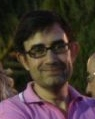
\includegraphics[width = 27mm]{JJM.jpg},] 
\noindent\emph{JJ Merelo} es catedrático de Universidad
en el área de Arquitectura y Tecnología de Computadores, y
actualmente director de la Oficina de Software Libre de la UGR.
Mantiene un blog desde el año 2002, y lo ha utilizado en clase desde
el año 2004; también wikis, agregadores y repositorios de código
como herramientas docente. Últimamente le ha dado por el \textsl{flipped
learning}, de lo que se informará debidamente en esta columna.
\end{window}}}

\medskip

{\small{\begin{window}[0,r,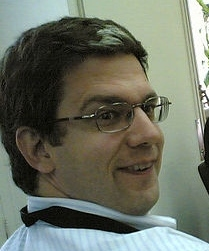
\includegraphics[width = 27 mm]{FTricas1.jpg},]
		\noindent \emph{Fernando Tricas García} es profesor
		titular de Lenguajes y Sistemas Informáticos del Departamento
		de Informática e Ingeniería de Sistemas de la Universidad de
		Zaragoza.  Empezó a estudiar la blogosfera casi cuando aún no
		existía (allá por el año 2002) y a tratar de integrarla en los
		cursos y tareas docentes un poco después.  Ha impartido
		numerosas charlas relacionadas con el tema de la Web 2.0, 
		internet y universidad,\ldots\ 
		Es actualmente Vicerrector de Tecnologías de la Información y
de la Comunicación.   
		\end{window}}}
%-------------------------------------------------




\noindent 
\bigskip

\noindent\emph{Todas las columnas de la serie Docencia 2.0
pueden descargarse en formato LaTeX desde
\surl{https://github.com/ReVision-Docencia-20/Columnas}}

\noindent\rule{90mm}{1pt}

{\small \noindent
\includegraphics[height = 4ex]{../CC.jpg} 2017 JJ. Merelo, F. Tricas. Este artículo es de acceso libre distribuido bajo los términos
de la Licencia Creative Commons de Atribución, que permite copiar,
distribuir y comunicar públicamente la obra en cualquier medio, sólido
o electrónico, siempre que se acrediten a los autores y fuentes
originales}

\end{multicols}
\end{document}
